\documentclass[9pt]{beamer}
\usepackage{styles/mypreamble}
%~~~~~~~~~~~~~~~~~~~~~~~~~~~~~~~~~~~~~~~~~~~~~~~~~~~~~~~~~~~~~~~~~~~~~~~~~~~~~~
\title{Алгоритмы машинного обучения}
\subtitle{Лекция 9. Линейная регрессия}
\author{Владимир Кукушкин}
\institute{СПбГЭУ - 2020}
\date{\today}
%~~~~~~~~~~~~~~~~~~~~~~~~~~~~~~~~~~~~~~~~~~~~~~~~~~~~~~~~~~~~~~~~~~~~~~~~~~~~~~

\begin{document}

\titlepage

\section{Постановка задачи}
\subsection{Одномерный случай}

\begin{frame}{Постановка задачи}
\begin{itemize}
    \item Пусть есть случайные величины $x$ и $y$ и выборки $(x_1, \ldots, x_n)^T$ и $(y_1, \ldots, y_N)^T$. 
    \item Предполагаем что $x$ и $y$ связаны линейной зависимостью $y=ax+b$.
    \item Как по выборке $x_i$, $y_i$ найти $a$ и $b$?
\end{itemize}
\begin{center}
    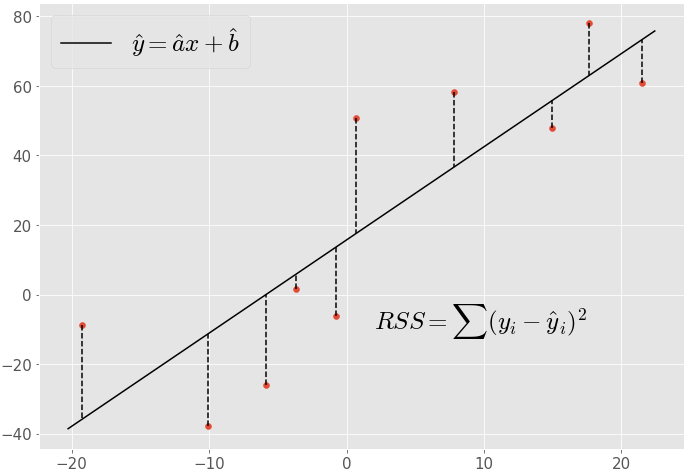
\includegraphics[height=0.5\textheight]{img/linear_regression_2d.png}
\end{center}
\end{frame}

\begin{frame}{Точное решение}
    $$\hat a, \hat b = \underset{a, b\in \mathbb{R}}{\mathrm{arg\;min}}\underbrace{\sum_{i=1}^N (y_i - (ax_i + b))^2}_{RSS}.$$
    $$\frac{\partial \text{RSS}}{\partial a} = 2\sum (y_i - ax_i - b)x_i\;\;\;\;\;\frac{\partial \text{RSS}}{\partial b} = 2\sum (y_i - ax_i - b)$$
\begin{itemize}
    \item Точное решение:
    $$\hat a = \frac{\overline{xy} - \bar x\bar y}{\overline{x^2} - (\bar x)^2} = \rho(x, y)\frac{\sigma_y}{\sigma_x} , \;\;\;\;\;\; \hat b = \bar y - \hat a \bar x$$
\end{itemize}
\end{frame}

\begin{frame}{Геометрическая интерпретация}
\begin{center}
    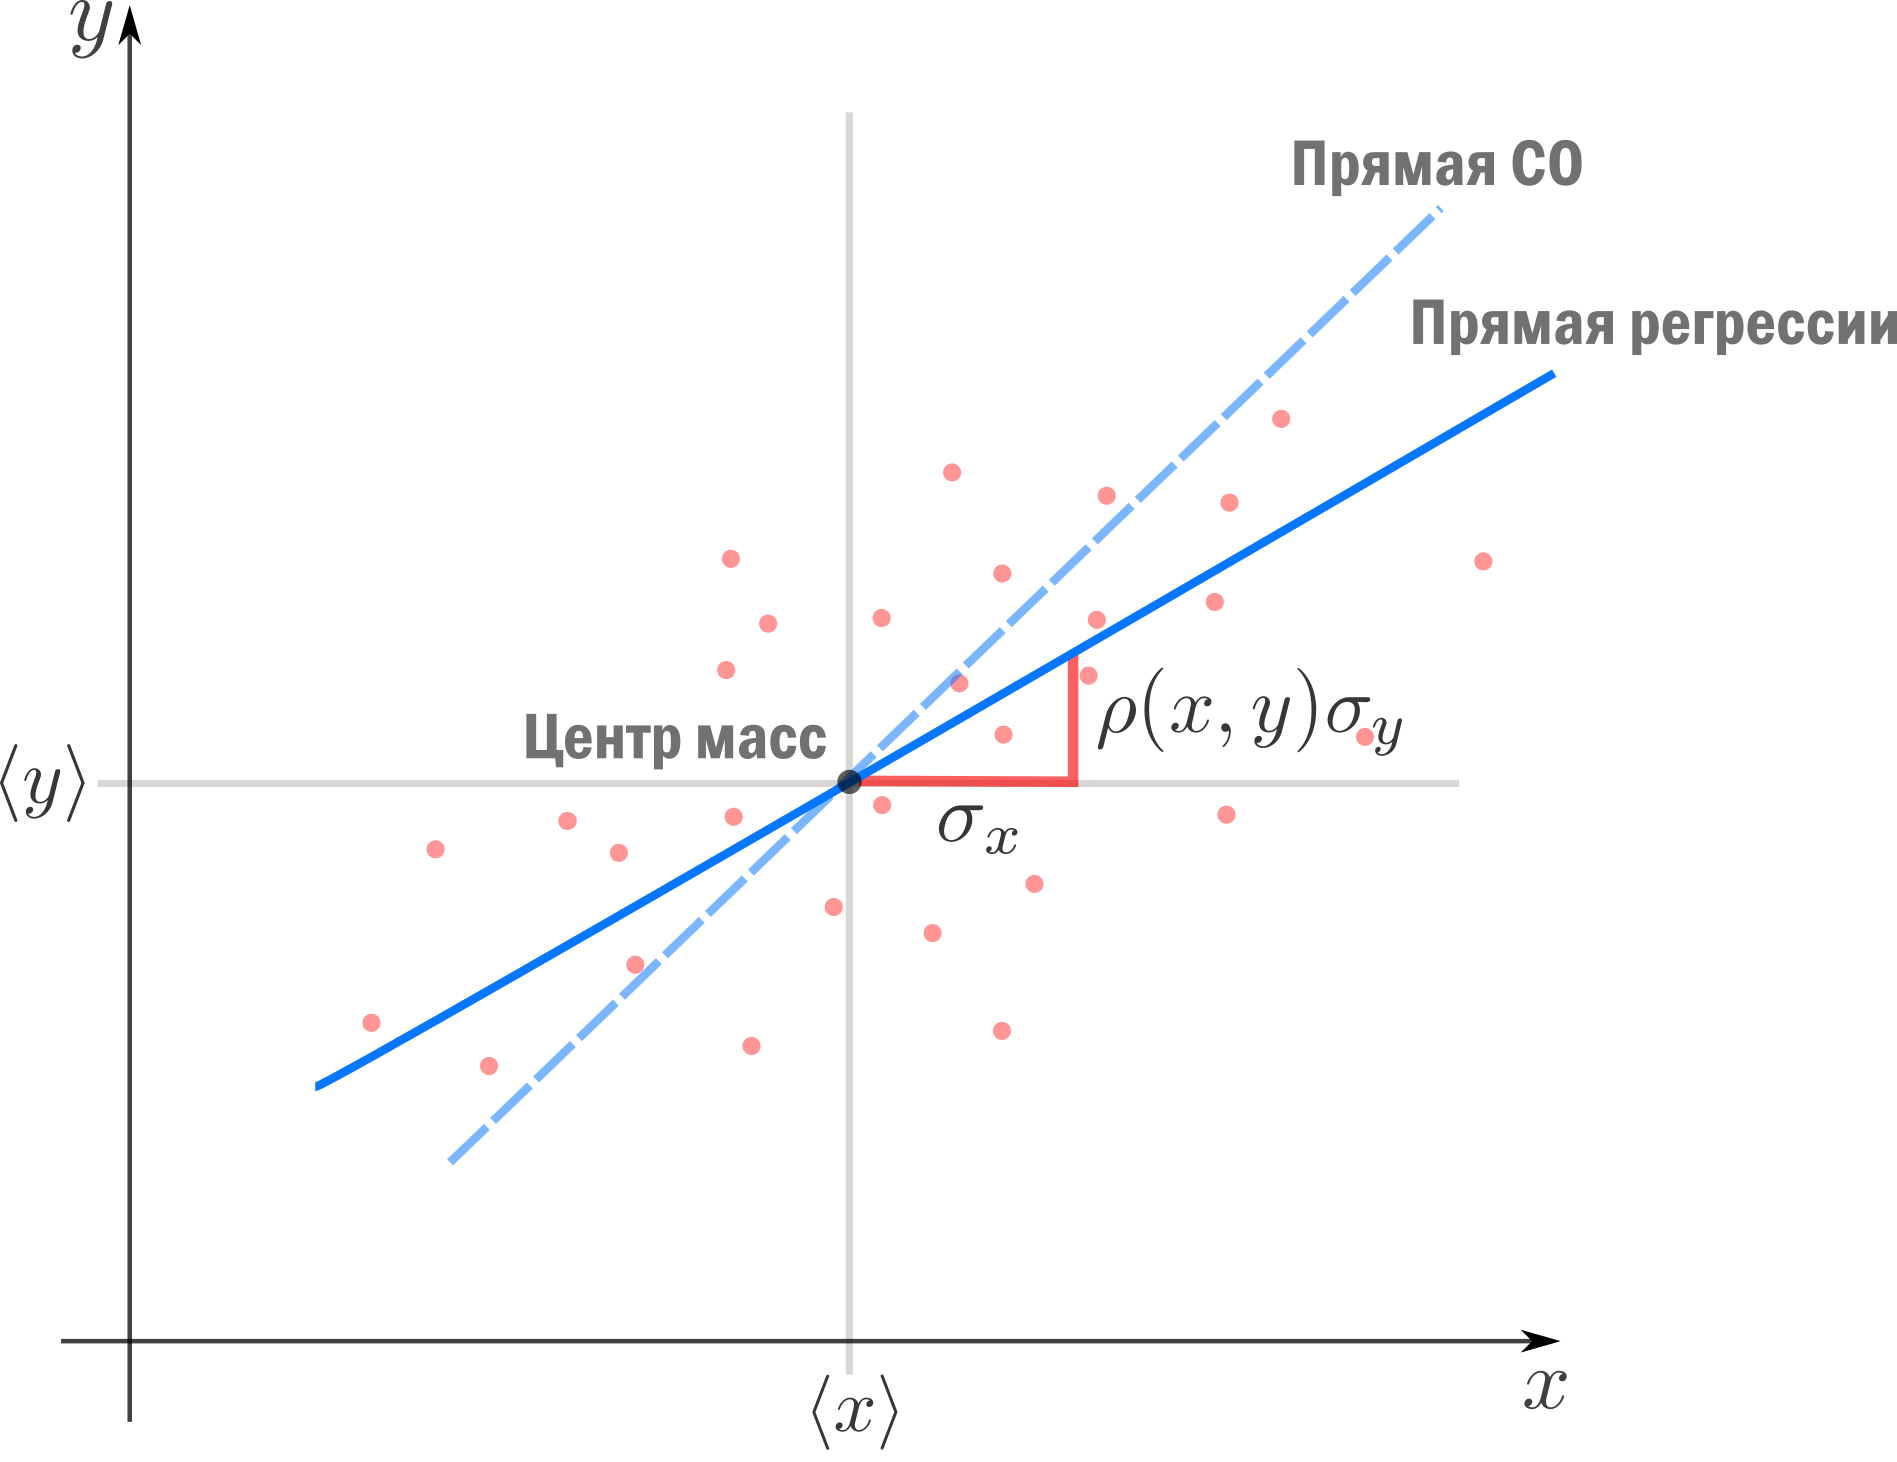
\includegraphics[height=0.5\textheight]{img/linear_regression_geometric_interpretation.png}
\end{center}
\begin{itemize}
    \item Регрессионная прямая проходит через центр масс.
\end{itemize}
\end{frame}

\begin{frame}{Историческая справка}
\begin{itemize}
    \item Гальтон. 1886 год. Изучал зависимость роста детей от роста родителей.
    \item В своей работе под регрессией он понимал тот факт, что рост детей отклоняется от их среднего меньше, чем рост родителей от их среднего.
    \item Впоследствии под регрессией стали понимать общий класс задач, который мы и проходим.
\end{itemize}
\begin{center}
    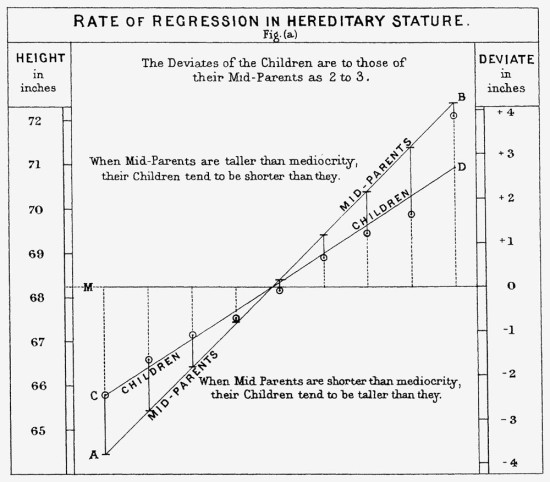
\includegraphics[height=0.6\textheight]{img/linear_regression_galton.jpg}
\end{center}
\end{frame}

\subsection{Многомерный случай}

\begin{frame}{Постановка задачи}
\begin{itemize}
    \item Пусть у нас есть матрица объект-признак $N\times p$: $X = (X_1,\ldots,X_p)$, где $X_i$ – столбцы фичей. Пусть $y$ – таргетный столбец.
    \item Хотим искать приближение $\hat y$ в виде:
    $$\hat y =\beta_0 + \sum_{j=1}^p X_j\beta_j \approx f(x),$$
    где $\beta = (\beta_0,\beta_1,\ldots,\beta_p)^T$ – коэффициенты регрессии.
    Добавим к $X$ единичный столбец и переобозначим
    $$X = \begin{pmatrix} 1&x_{11}&\ldots&x_{1p}\\1&x_{21}&\ldots&x_{2p}\\\cdots&\cdots&\ddots&\cdots\\1&x_{N1}&\ldots&x_{Np}\\ \end{pmatrix}.$$
    Тогда $\hat y = X\beta$.
    \item Функция ошибки: RSS.
\end{itemize}
\end{frame}

\begin{frame}{Точное решение}
    \begin{itemize}
        \item $\text{RSS}(\beta) (y-X\beta)^T(y- X\beta)$
        $$\frac{\partial \text{RSS}}{\partial \beta} = -2X^T(y-X\beta),\;\;\;\;\;\;\;\;\;\frac{\partial^2 \text{RSS}}{\partial \beta\partial\beta^T} = -2X^TX.$$
        \item Предполагаем, что $X$ полного ранга. Отсюда $X^TX$ положительно определена. Тогда RSS выпуклая, а значит минимум находится в точке
        \begin{equation}\label{linreg_projection}
            X^T(y-X\beta) = 0.
        \end{equation}
        \item Итоговое решение:
        \begin{equation}\label{linreg_hat_beta}
            \hat \beta = (X^TX)^{-1}X^Ty,    
        \end{equation}
        \begin{equation}
            \hat y = X(X^TX)^{-1}X^Ty.
        \end{equation}        
        \item Такой подход называется методом наименьших квадратов (МНК).
    \end{itemize}
\end{frame}

\begin{frame}{Геометрическая интерпретация}
\begin{itemize}
    \item Минимизация RSS эквивалентна минимизации $\|y - X\beta\|^2$.
    \item Если все столбцы матрицы линейно-независимы, то они образуют базис некоторого $p+1$-мерного пространства $\mathcal{C}$.
    \item Если $\mathcal{C}^\perp$ -- ортогональное дополнение к нему, тогда $\mathbb{R}^N = \mathcal{C} \oplus \mathcal{C}^\perp$ и $y = y_{\text{proj}} + y_\perp$.
    \item В силу (\ref{linreg_projection}), $y_{\text{proj}} = \hat y$.
\end{itemize}
\begin{center}
    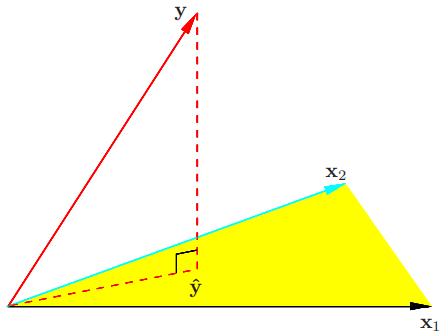
\includegraphics[height=0.5\textheight]{img/linear_regression_projection.png}
\end{center}
\end{frame}

\section{Статистические свойства коэффицициентов регрессии}

\begin{frame}{Статистическая постановка задачи}
    \begin{itemize}
        \item Предполагаем, что $y = X\beta + \varepsilon$, где $\varepsilon \sim \mathcal{N}(0, \sigma^2)$. То есть случайный шум искажает реальную зависимость $y=X\beta$. Важно: шум несмещённый (центр в нуле) и имеет постоянную дисперсию $\sigma^2$.
        \item $\hat \beta$ из МНК (\ref{linreg_hat_beta}) можно считать оценкой истинных параметров $\beta$: $\hat \beta = (X^TX)^{-1}X^Ty$.
        \item Матожидание:
        $$E(\hat \beta) = E((X^TX)^{-1}X^T(X\beta + \varepsilon)) = \beta.$$
        \item Вспомним, что для любой матрицы $A$: $Var(Ay)$ = $A Var(y) A^T$. Тогда: 
        \begin{multline*}
            Var(\hat\beta) = (X^TX)^{-1}X^T \underbrace{Var(y)}_{\sigma^2 I} X\underbrace{((X^TX)^{-1})^T}_{(X^T X)^{-1}}=\\
            = \sigma^2 (X^TX)^{-1}(X^TX)(X^TX)^{-1} = \sigma^2 (X^TX)^{-1}.
        \end{multline*}
        \item Значит, $\hat \beta \sim \mathcal{N}(\beta, \sigma^2(X^TX)^{-1})$.
    \end{itemize}
\end{frame}

\begin{frame}{Теорема Гаусса-Маркова}
    \begin{itemize}
        \item Теорема гарантирует то, что МНК-коэффициенты регрессии имеют наименьшую дисперсию среди всех линейных несмещённых оценок.
    \end{itemize}
\end{frame}

\begin{frame}{Свойства остатков}
\begin{itemize}
    \item \href{https://stats.stackexchange.com/questions/76738/proof-that-regression-residual-error-is-an-unbiased-estimate-of-error-variance}{Можно показать}, что $\hat\sigma^2 = \frac{1}{N - p - 1}\sum_{i=1}^N(y_i - \hat y_i)^2$ является несмещённой оценкой.
    \item Ещё \href{https://stats.stackexchange.com/questions/20227/why-is-rss-distributed-chi-square-times-n-p/20230\#20230}{можно показать} что $\hat \sigma^2 \sim \frac{\sigma^2}{N-p-1}\chi^2_{N-p-1}$.
\end{itemize}
\end{frame}

\begin{frame}{Значимость коэффициентов}
    \begin{itemize}
        \item H0: $\beta_j = 0$.
        \item H1: $\beta_j \neq 0$.
        \item $z_j = \frac{\hat\beta_j - \beta_j}{\hat\sigma\sqrt{v_j}},$ где $v_j$ – $j$-й диагональный элемент матрицы $(X^TX)^{-1}$.
        \item Если H0 справедлива, то $z_j\sim t_{N-p-1}$.
        \item То есть можно посчитать статистику $z_j$, сравнить с критическими значениями $t_{N-p-1}$ и отвергнуть/не отвергнуть гипотезу.
        \item Доверительный интервал для $\beta$: $$(\hat\beta_j - t_{1-\alpha/2}\hat\sigma\sqrt{v_j}, \hat\beta_j - t_{1-\alpha/2}\hat\sigma\sqrt{v_j}).$$ Проверить, лежит ли в нём ноль.
    \end{itemize}
    Проверка таких гипотез позволяет произвести отбор фичей (a.k.a. feature selection) и удалить из датасета фичи, которые не несут сигнала. При этом нужно проверить, что после их удаления качество модели не просело.
\end{frame}

\begin{frame}{Значимость группы коэффициентов}
    \begin{itemize}
        \item Хотим проверить значимость не одной фичи, а группы фичей. Например, это может быть бинаризованная категориальная фича.
        \item Проверяем, что будет, если убрать все её бинарные фичи?
        \item H0: $\beta_j = 0$ (для всех $j$ из группы фичей).
        \item H1: $\beta_j \neq 0$.
        \item $F=\frac{(RSS_0 - RSS_1)/(p_1-p_0)}{RSS_1/(N-p_1-1)},$
        \item где $RSS_1$ полная модель с $p_1$ фичами, $RSS_0$ – усечённая модель с $p_0$ фичами.
        \item Если справедлива H0, то $F\sim F_{p_1-p_0, N-p_1-1}$.
    \end{itemize}
\end{frame}

\section{Оценка качества регрессионной модели и интерпретация коэффициентов}

\begin{frame}{Дисперсионное разложение}
\begin{itemize}
    \item $\sigma^2_{reg} = ESS = \frac{1}{N}\sum_{i=1}^N (\hat y_i - \bar y)^2$: Explained Sum of Squares.
    \item $\sigma^2_{data} = TSS = \frac{1}{N}\sum_{i=1}^N (y_i - \bar y)^2$: Total Sum of Squares.
    \item $\sigma^2_{res} = RSS = \frac{1}{N}\sum_{i=1}^N (y_i - \hat y_i)^2$: Residual Sum of Squares (напоминание).
    \item Тогда (\href{https://en.wikipedia.org/wiki/Explained_sum_of_squares\#Simple_derivation}{см. доказательство})
    \begin{equation}\label{linreg_variance_decomposition}
        \sigma^2_{data} = \sigma^2_{reg} + \sigma^2_{res}.
    \end{equation}
\end{itemize}
\begin{center}
    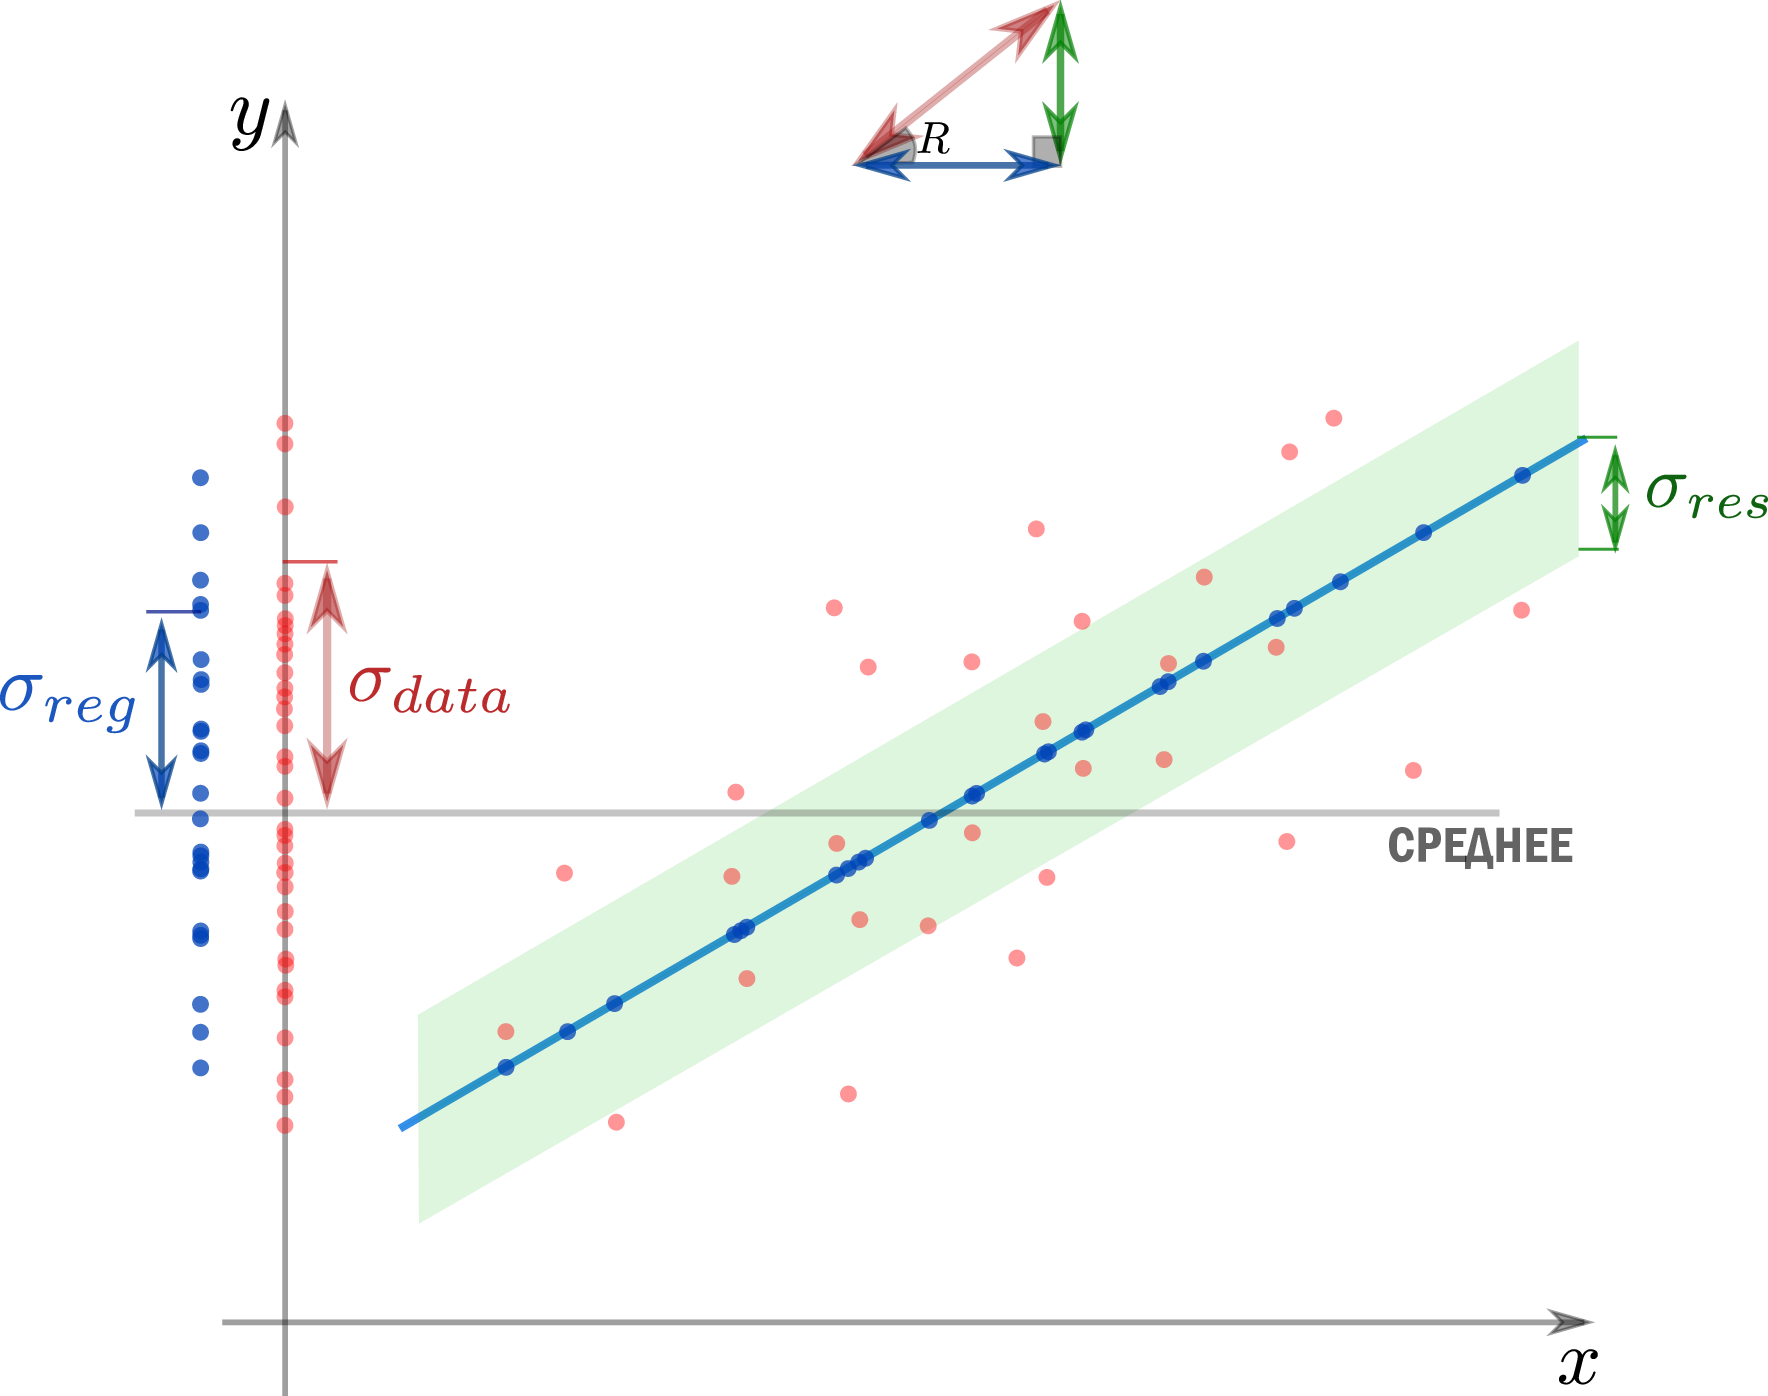
\includegraphics[height=0.55\textheight]{img/linear_regression_tss_ess_rss.png}
\end{center}
\end{frame}

\begin{frame}{Коэффициент детерминации}
    \begin{itemize}
        \item У хорошей модели дисперсия остатков должна быть мала по сравнению с дисперсией таргетной переменной.
        \item $R^2 = 1 - \frac{RSS}{TSS} = \frac{ESS}{TSS}$: доля объяснённой вариации. 
        \item $0 \leq R^2 \leq 1$. Чем ближе к 1, тем лучше.
        \item Дополнительный физический смысл. Пусть $\tilde a(x) = \bar y$: бейзлайн-модель. Тогда $TSS = RSS(\tilde a)$ и $R^2 = 1 - \frac{RSS(\hat a)}{RSS(\tilde a)}$. То есть коэффициент детерминации показывает, во сколько раз МНК-модель лучше, чем средняя константная.
    \end{itemize}
\end{frame}

\begin{frame}{Коэффициент детерминации. Геометрическая интерпретация.}
\begin{center}
    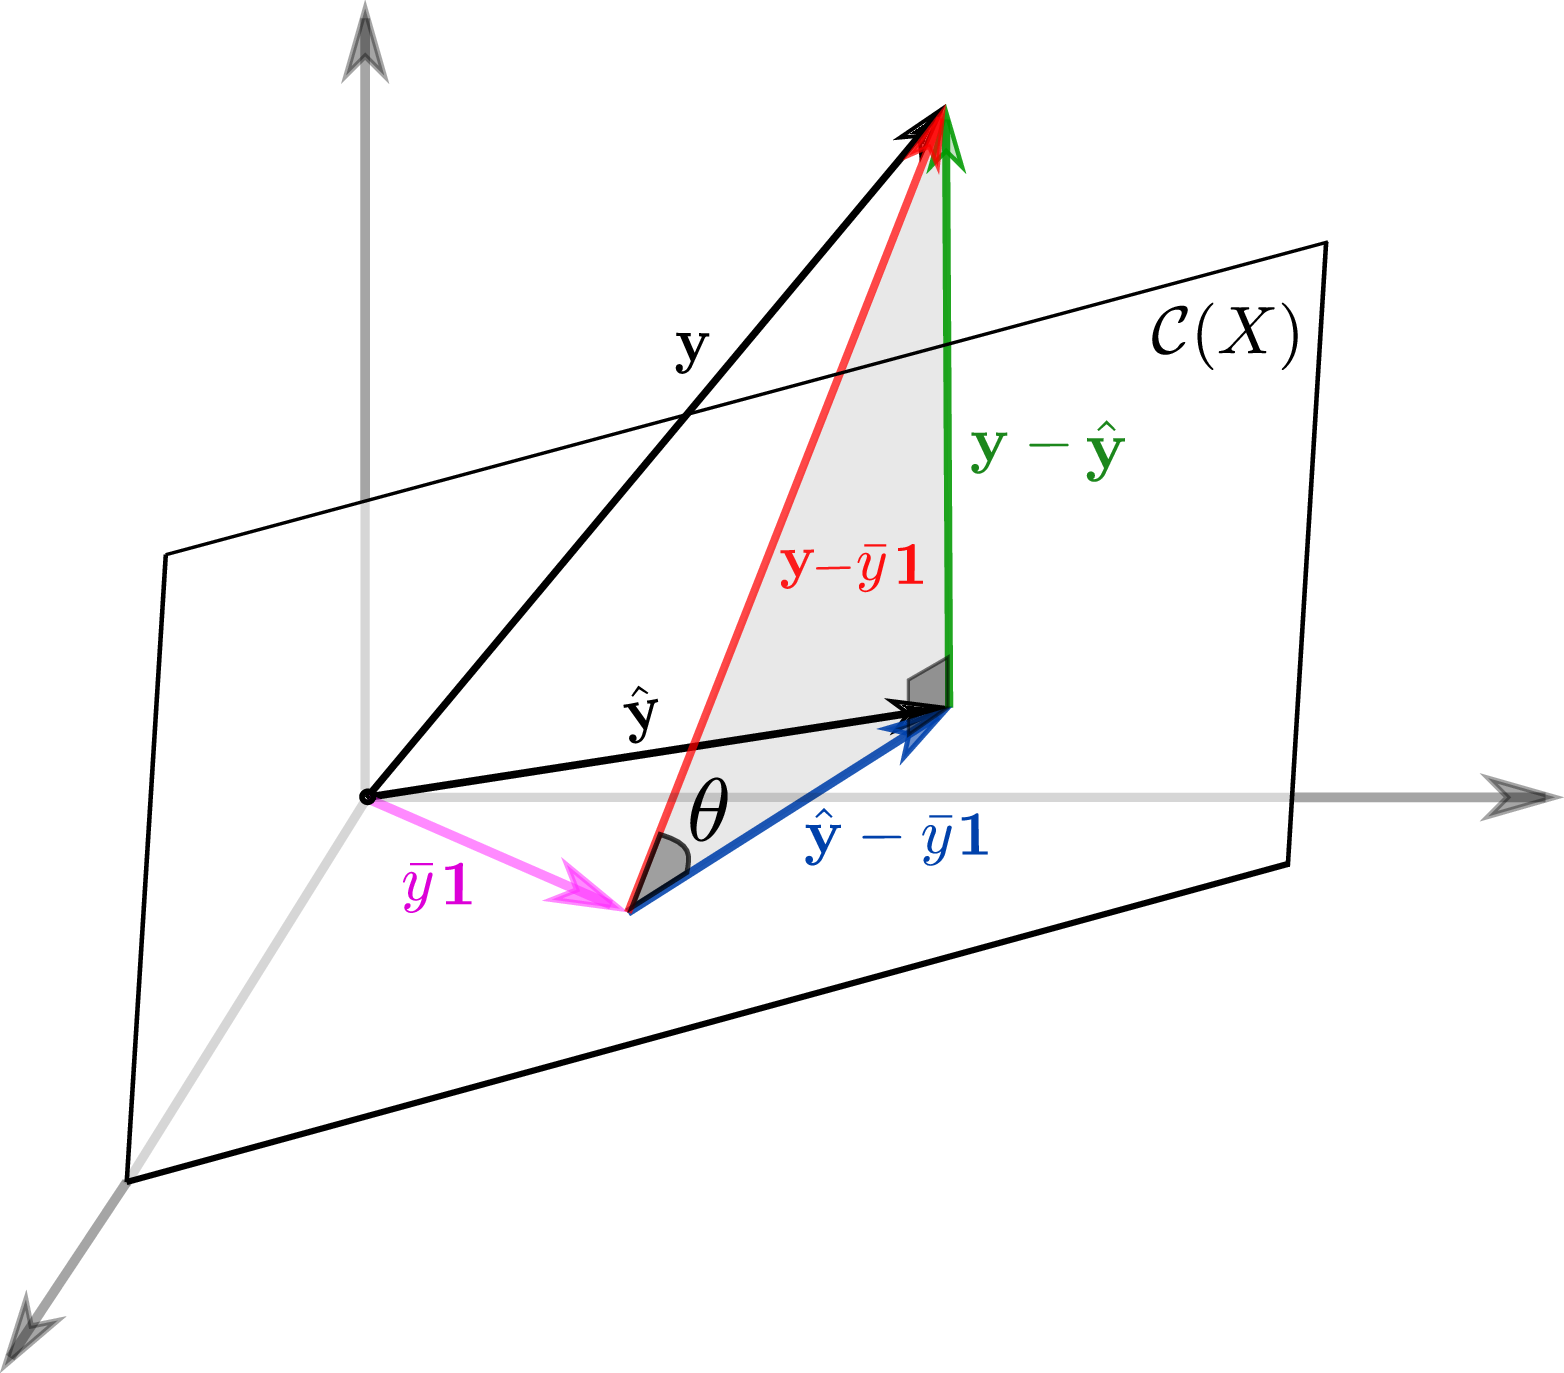
\includegraphics[height=0.5\textheight]{img/linear_regression_determination_coefficient.png}
\end{center}
\begin{itemize}
    \item $\bar y\textbf{1}$ -- N-мерный вектор из средних значений.
    \item Аналог разложения дисперсии (\ref{linreg_variance_decomposition}):
    $$\|y-\bar \bar y\textbf{1}\|^2 = \|y-\hat y\|^2 + \|\hat y - \bar y\textbf{1}\|^2.$$
    \item Отсюда $R^2 = \frac{\|\hat y - \bar y\textbf{1}\|}{\|y-\hat y\|} = \cos^2\theta$.
\end{itemize}
\end{frame}

\begin{frame}{Adjusted $R^2$}
    \begin{itemize}
        \item Недостаток $R^2$: растёт вместе с увеличением сложности модели. Поэтому некорректно сравнивать по $R^2$ модели, настроенные на разном количестве фичей.
        \item Adjusted $R^2$ устраняет этот недостаток. Он включает штраф за дополнительно включённые признаки.
        $$R^2_{adj} = 1 - \frac{RSS/(N-1)}{TSS/(N-p)}$$
        \item $R^2_{adj} < 1$. Теоретически может быть меньше нуля, но только при маленьком $R^2$ и большом количестве фичей.
    \end{itemize}
\end{frame}

\begin{frame}{Интерпретация коэффициентов}
\begin{itemize}
    \item На сколько единиц изменится таргет при изменении предиктора на одну единицу.
\end{itemize}
\end{frame}

\section{Плюсы, минусы, подводные камни}
\begin{frame}{Квартет Анскомба}
    \begin{center}
        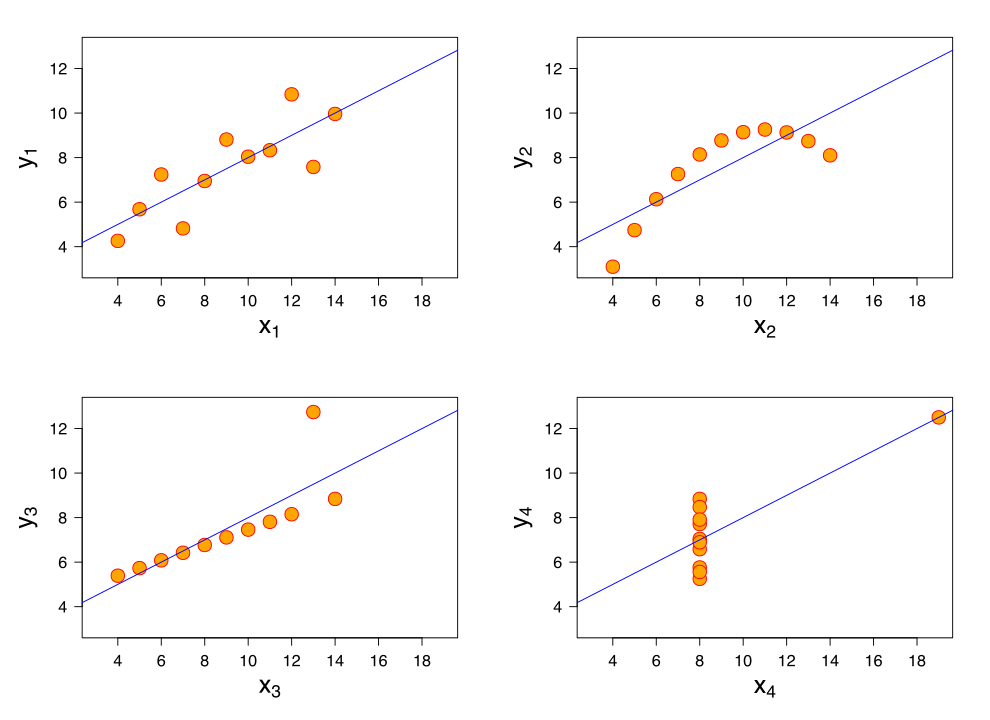
\includegraphics[height=0.7\textheight]{img/linear_regression_anscombes_quartet.png}        
    \end{center}
    На всех четырёх графиках $R^2$ один и тот же!
\end{frame}

\begin{frame}{Мультиколлинеарность}
    \begin{itemize}
        \item На практике коррелирующие фичи встречаются очень часто.
        \item Как правило, проявляется это в том, что у матрицы $X^TX$ будет большое число обусловленности, и обратная $(X^TX)^{-1}$ будет содержать огромные по модулю значения.
        \item Коррелирующие фичи можно отсеивать вручную.
        \item А можно использовать, например, градиентный спуск. Искать $\hat beta$, минимизирующие RSS.
        \item Но лучше использовать регуляризацию, о которой поговорим в следующей лекции.
    \end{itemize}
\end{frame}

\begin{frame}{Нелинейные модели, сводящиеся к линейным}
К предикторам и отклику можно применять различные нелинейные функции, оставляя модель линейной по $\beta$. Примеры (для одной переменной $x$):
    \begin{itemize}
        \item Сводятся к линейной модели через замену переменной:
        \begin{itemize}
            \item $y = \beta_0 + \beta_1\frac{1}{x} + \varepsilon$,
            \item $y = \beta_0 + \beta_1\ln x + \varepsilon$,
            \item $y = \beta_0 + \beta_1 x^\alpha + \varepsilon$.
        \end{itemize}
        \item Мултьтипликативная модель: $y = \alpha x^\beta\varepsilon$. Сводится к $\ln y = \ln\alpha + \beta\ln x + \ln \varepsilon$. В этом случае $\ln \varepsilon \sim \mathcal{N}(0, \sigma^2)$.
        \item Экспоненциальная модель: $y = \alpha e^{\beta x}\varepsilon$. Сводится к $\ln y = \ln\alpha + \beta x + \ln \epsilon$.
        \item Обратная модель: $y = \frac{1}{\beta_0 + \beta_1 x + \varepsilon}$. Сводится к $\frac{1}{y} = \beta_0 + \beta_1 x + \varepsilon$.
    \end{itemize}
\end{frame}

\begin{frame}{Заключение}
\begin{itemize}
    \item Очень понятный алгоритм как по построению, так и по интерпретации.
    \item Коррелирующие фичи всё портят.
    \item Неустойчив к выбросам.
    \item Определяет только линейную зависимость.
    \item Обращение матрицы $(X^TX)^{-1}$ имеет кубическую сложность.
\end{itemize}
\end{frame}

\begin{frame}[allowframebreaks]
    \frametitle{Литература}
    \bibliographystyle{unsrt}
    \nocite{esl, linreg_habr}
    \bibliography{references.bib}
\end{frame}
\end{document}